\chapter{Measuring control in hypergraphs}

Hierarchical production organisations are often characterised by a distinction between ownership and control \citep{JensenMeckling1976, FamaJensen1983}. This separation leads to a distinction between the roles of `shareholders' and the `directors' within a firm. Shareholders and directors can own and control many firms across many different industries of the economy. As such, a set of firms can have \emph{overlapping} and \emph{interlocking} directorates depending on how their directors form memberships to multiple firms within the set. Note that we consider an overlapping directorate and an interlocking directorate as different notions. When a director sits on the boards of multiple firms we suggest that the directorates of these firms `overlap' due to the presence of at least one identical director. If firm $A$ has an overlapping directorate with firm $B$, and firm $B$ has an overlapping directorate with some other firm $C$ then we claim that firms $A$ and $C$ are `interlocked' due to their mutual overlap with firm $B$'s directorate. According to the definition of the interlocks during the time in which they were initially debated, the directorate of firms $A$ and $C$ need not overlap for there to be an interlock; it must simply be that directors from firm $A$ and firm $C$ be connected by some intermediary in which they both have a mutual overlap with.

The structure of interlocking and overlapping directorates has gained much interest in both industry and academia over the past century. This research has focused on the relationship between overlapping and interlocking directorates, the positional power of well-connected firms and directors, and the spread of corporate governance through sprawling directorate networks \citep{RoyBonacich1988}. The consequence of the research is a raft of accepted stylised facts and policy implications suggesting that tightly-knit directorate networks within an industry, and between related industries, is an uncompetitive practice. The epitome of this being the unbridled power of J.P. Morgan and his associates. This chapter uses novel methodology in network theory to test the stylised facts surrounding interlocking directorates during the height of Morgan's influence. Specifically, by using directorate data we elaborate on the actions of network entrepreneurship within a platform economy using the example of New York City at the beginning of the twentieth Century. We also feed the notion of network entrepreneurship into a discussion of institutional entrepreneurship by elaborating on how the capitalists at the time forced a change to the institutional design of American business. Furthermore, the chapter finds that whereas the number of interlocks are largely irrelevant for a firms performance, the weights and context of the interlocks matters significantly to the profitability of the firm.

\subsubsection{J.P. Morgan and the \emph{Money Trust}}

The structure and potential influence of directorate networks were brought to the fore within industry in 1912 when the United States House Committee on Financial Services organised a special committee---named the \emph{Pujo Committee}---to investigate a so-called `Money Trust'. This was seen to be a \emph{de facto} monopoly of control by a handful of financial institutions and bankers across multiple industries. Specifically, John Peirpont Morgan and his financial institution, J.P. Morgan \& Co., were accused of holding and exercising excessive economic power across the United States of America through directorial ties and shareholdings in other firms. The hearing concluded in 1913 and Morgan was found capable of exercising monopoly power over a number of industries---including the railway industry, the financial services industry and insurance---and exercising excessive bargaining power when writing contracts through his own shareholdings and board memberships, and the board memberships of his employees of J.P. Morgan \& Co \footnote{Evidence of the investigation can be found at \href{https://fraser.stlouisfed.org/title/?id=80}{https://fraser.stlouisfed.org/title/?id=80}.}.

The outcome of this investigation lead to the passing of the \emph{Federal Reserve Act of 1913} and the \emph{Clayton Antitrust Act of 1914}. The Federal Reserve Act immediately lead to the establishment of the Federal Reserve Central Bank; which had been discussed for several years prior to the investigation as a reaction to the panics of 1907 and 1911 \citep{Silber2007}. The Clayton Antitrust Act, built upon the Sherman Antitrust Act of 1890, was an effort to reduce monopolisation and other anti-competitive practices such as price discrimination, exclusive dealing agreements, tying agreements, and mergers and acquisitions that would reduce market competition. Title 15, Chapter 1, Section 19 of this Act concerned interlocking directorates and officers. It aimed to reduce the number of overlapping and thus interlocking directorates of competing firms within the same industry and across industries. Although the law was not strictly enforced, it gradually lead to a weakening of the American directorial elite throughout the early and mid twentieth Century \footnote{Note, however, that other social and economic phenomena occurred during this time which would dilute the power of directors, such as a developing stock market and social, economic, and financial globalisation}. This was indeed a pivotal time in financial and economic history throughout the developed world. These anticompetitive institutions were later adopted by other economies, including in the UK, where there had been a swathe of industrial mergers and acquisitions in the financial and railway industry. Undeniably Morgan, and those associated with him and his company, had some power over the economic success of others.

One of Morgan's known interests was the establishment of the Northern Securities Company in 1901
\citep{Langdell1903}. The company was a railroad trust specifically purchasing shares of other important railroad companies, such as the Burlington and Quincy Railroad, which was a vital railroad hub in Chicago. The reason for its establishment was in response to a bidding war between Hill, Morgan, and Edward H. Harriman, the then President of the Union Pacific Railroad, for the shares of Northern Pacific Railway, owned by Hill and Morgan. Subsequently this bidding war transferred into competition for the shares of Burlington and Quincy Railroad. Hill created the Northern Securities Company to control all three railroads. The company was established and capitalised at \$400 million, with James J. Hill serving as its President, who was also the President of the Great Northern Railway.

The establishment of the company was considered by the Department of Justice as being anti-competitive, specifically breaching the Sherman Antitrust Act of 1890. There were multiple reasons as to why the Northern Securities Company was seen to be anti-competitive: first, due to a \emph{de facto} monopolisation through merger from a harmonisation of incentives and cooperation between directors of multiple rival railway companies; second, diluting competition regarding the the purchasing of shares of other railroad companies; and third, it reduced the potential for new competitor railroads that could easily be subsumed by the Northern Securities Company. In 1904 the Department of Justice ruled five votes to four in favour of dissolving the Northern Securities Company. This was one of the first uses of the Sherman Act, and set the foundation for 44 other Federal Antitrust cases.

This was an important time in the development of the United States and the mentality surrounding mergers, monopolies, and overlapping directorates. However, in general, regulation was lax surrounding the structure of directorate networks. It is therefore interesting to see whether the structure of the directorate network is reflective of economically powerful and anti-competitive practices, and to develop measures in an effort to identify powerful and influential directors and firms.

\medskip\noindent This chapter follows on from the discussion of network and institutional entrepreneurship, and previous interest in the structure of directorate networks. We also research whether the control of a firms' directorate has an impact on its economic performance. To answer this we develop a bespoke measure---the $\sigma$-score---which regards the control of individual directors and firms. Moreover, we characterise elite directors and assess whether the presence of so-called \emph{elites} within a firm has an impact on its performance.

Two issues of identification and measurement are resolved in this chapter. The first pertains to the identification of nodes and affiliations that have control in a directorate network, which is represented in the most general context as a \emph{hypergraph}. A hypergraph is a generalisation of a network that contains a set of links and a set of nodes. In a hypergraph a link---called a \emph{hyperlink}---can connect to multiple nodes, suggesting that all nodes are connected with each other. This provides a good setting for defining boards of directors whereby a node represents an individual director and a hyperlink represents a firms. From this we test whether a firms control has causality on its economic performance. The second pertains to the identification of elites; nodes that are embedded in all aspects of a socio-economic space. Due to their multiplicity of embeddedness and their ability to directly gather and use diverse and complimentary information we assess whether the presence of elites organise the evolution of the directorship network over time. Whereas the $\sigma$-score is a degree-based centrality measure, and therefore increases in a strictly monotonic fashion with the degree of the node, the measure of elites is not.

The process of parsing out sets of elites uncovers an \emph{elite network structure} whereby elites are connected through all aspects of the network. From the resulting elite network structure we assess elite power through brokerage measures and identify important subsets of nodes who hold controlling positions within elite structures, possessing some hierarchy over the set of elites. Using this information regarding the elites and influence of individual nodes and affiliations we use this information as inputs for a regression analysis that measures whether these factors have an impact on the value of a firms assets. There are a number of derived questions, such as whether the influence and connectivity of a financial institution has an impact on their lending, borrowing, and stability over time.

In this chapter we further argue that networks regarding firm directorships lend themselves to a multidimensional analysis. In such networks we consider a dimension to be equivalent to a specific industry of an economy. How related dimensions are measured by the nodes embedded within them and the consistency of the linkages between the nodes. Power between dimensions is therefore held by nodes that have access to information between them.

\paragraph{Chapter outline.}

First, we provide a literature review on the interaction between how connected directorates are within firm boards and the firms performance. Section~\ref{Theory:Influence} introduces hypergraphs, networks, and other preliminary concepts. The section then provides some bespoke ways in which to measure the influence of individual nodes and affiliations in hypergraphs and network projections. Section~\ref{Theory:Elites} introduces aspectual hypergraphs, analyses and provides measures for the relatedness between aspects, and finally defines elites and elite structures.

\section{Corporate connectivity and firm performance} \label{Literature}

Economics and sociology have investigated the relationship between an individuals' social structure and their economic outcomes \citep{Granovetter1985}. This literature includes analysis into the diffusion and adoption of innovation \citep{Coleman1966}, coalition formation \citep{Kapferer1969}, elite decision making and community structure \citep{LaumannGalaskiewiczMarsden1978}, information diffusion in labor markets \citep{Granovetter1973}, and decisions regarding the level of education that an individual pursues and whether or not to undertake criminal activity \citep{BallesterZenou2006, Jackson2007}. The types of networks examined in these papers include social communities, powerful families and political and economic systems \citep{Padgett1993, Padgett1994}. More recently, \citet{Banerjee2013} discussed the social structure regarding the diffusion of micro-finance practices that depends on the structure of society.

%%

There have been numerous studies on the social structure produced by members of boards of directors. For example, \citet{Levine1972} documents the existence of interlocked directorates between the boards of major banks and the boards of major industrials. Related to our study, \citet{Dooley1969} observes that an industrial company whose board is occupied by a banker can obtain capital at favourable rates. Much of this prior research documents how particular interlocks are created \citep{PfefferSalancik1978}, how they are maintained \citep{Palmer1983, PalmerFriedlandSingh1986}, the density or centrality of the network \citep{DavisYooBaker2003}, and the stability of the network though time \citep{BeckmanHaunschildPhillips2004}. However, relatively little work documents the economic consequences of these board networks on firm performance.

The association between a firm's centrality, connectedness, or importance in the interlocking boardroom network is ex-ante theoretically ambiguous. There is an abundance of arguments within organisational sociology and economics on why companies with well-connected boards may benefit from their position in the network. First, interlocking boardroom networks allow firms to improve the terms of contracts between firms \citep{SchoormanBazermanAtkin1981}. Second, because directors have important knowledge and contacts, being central in the boardroom network gives a firm better access to such useful knowledge, contacts and resources, which can benefit firms and particularly those that operate in uncertain business environments \citep{Mol2001, NicholsonAlexanderKiel2004}. Third, being central in the interlocking boardroom network could also allow for more or better means of information exchange, leading to a reduction in the costs of obtaining information and perhaps improving business decisions \citep{Mizruchi1990}. Fourth, board connections also represent a mechanism through which value-improving business innovations can spread in this way, being central in a network can add value to a firm \citep{HaunschildBeckman1998}. Finally, interlocking boardroom networks may facilitate cartel formation, which can yield private economic benefits within the cartel by restricting competition.

However, there are also plausible reasons why connectedness in the board network can negatively impact a firm. First, the extent that being well-connected in the boardroom network involves having boardroom members that take on many boardroom jobs, a firm may suffer economically from the deteriorating quality if their directors work in the firm \citep{FichShivdasani2006, FichWhite2005}. Second, it is possible that misleading or incorrect information is spread though the board network. The problems of misinformation are heightened with more sprawling interlock networks. If this information is used for strategic choices, it can easily result in a decrease in shareholder value. Finally, although collusion can have a positive impact on shareholder value, the resulting regulatory, litigation, and reputation costs can produce substantial losses of shareholder value.

This chapter is related to an emerging body of literature in economics, finance, and sociology demonstrating the role of personal and social connections in the spread of information. The chapter also contributes to the literature providing a link between social networks and favourable economic outcomes. For example, \citet{HwangKim2009} and \citet{HwangKim2012} demonstrate that socially connected CEO's enjoy higher compensation and retention rates; \citet{FaccioMcConnellMasulis2006} establish that politically connected firms have a higher likelihood of receiving bailout assistance; and \citet{StuartYim2010} find that connected firms have a higher propensity to be targeted in mergers and acquisitions deals. Our findings corroborate and extend this literature by providing additional evidence of the influence of social networks on firm-level economic outcomes. Specifically, our results suggest that firms central in the broader interlocking boardroom network experience improved operating and stock price performance.

Some prior research has delved into similar empirical questions. \citet{EngelbergGaoParsons2013} demonstrates that firms with connections to capital suppliers enjoy more favourable terms of lending, improved credit ratings, and superior stock price performance. \citet{Boyd1990} finds that among firms facing a more uncertain business environment, those with more connections to other companies through interlocks tend to perform better in terms of sales improvements and return on equity. Using a sample of 350 Brazilian firms, \citet{SantosSilveiraBarros2009} find that firm value is negatively affected by interlocking boards, particularly boards with busy boards and firms in which CEO's hold directorships in other companies. 

% Similarly, \citet{NonFrances2007} find a negative relationship between the number of interlocks and future performance for a sample of 101 Dutch firms.

These past studies are important. However, we suggest that there is a limitation to using standard centrality measures when applying them to specific environments such as boards of directors. Indeed, the outcomes witnessed from using off-the-shelf measures may be different from alternative, purpose-built centrality measures. In this chapter we provide a measure of a nodes influence, which we argue can be appropriately applied to directorate networks; this is extended to find the influence of firms to which the directors are members of. Of interest is the importance and influence of elites: directors who have influence in multiple industries.

% De Long (1990) finds that J.P. Morgan and Co., and those organisations associated with Morgan and his men, benefited from persistent economic benefits in the form of around a $30\%$ increase in common stock equity value. Ramirez (1995) further finds that organisations associated with Morgan benefited from decreased liquidity constraints. Chernow (2010) chronicles the rise of the House of Morgan, elaborating on J.P. Morgan's ability to monopolise lending and forming de facto oligopolies within the railway industry.

%\subsection{Measures of centrality}

%Freeman (1977) and Bonahich (1972) were first to develop measures of network centrality that are still commonly used network science \footnote{For more information on commonly used node centrality measures consider Jackson (2008).}. The degree and eigenvector centrality measures provide the foundation for other centrality measures that have been subsequently developed. The most common, the degree centrality, is determined by the number of links a given node has, and the eigenvector centrality measure is determined by the number of links that a node has and the number of links that each of its neighbours have. PageRank centrality (Brin and Page, 1998) develops a measure that is built from eigenvector centrality; it specifically discounts the importance of a nodes link by the number of other connections the node has. These common measures of centrality have been applied to many different social and economic contexts, and have had application to directorate networks (Khanna et al., 2015; El-Khatib, 2015). Sims and Gilles (2014) provide a measure brokerage attached to a node set, which is related to the economic notion of contestability.

%Of specific interest to this chapter is the work of Brink and Gilles (1996; 2000). The authors develop a measure of node dominance, known as the $\beta$-measure, which provides an axiomatic generalisation of degree centrality in a directed network. The measure has had specific application to tournaments and games, but has yet to be applied to directorate networks. Borm, Brink, and Slikker (2002) develop an iterated $\beta$-measure which, much like the eigenvector and PageRank centralities, develops a score based on the dominance of the nodes that it dominates. Again, this lacks a specific application to directorate networks.

%When considering directorate networks, the analysis of how industries are connected through a directorate is important. It can reveal complementaries and information sharing between industries unobservable by assessing outputs alone. A directors ability to have influence and share information between industries can reveal some importance. Corominas-Murtra and Thurner (2014) develop a mechanism in which to identify the weak core and the structure of important nodes within a multidimensional network. Nodes that exist within a $k$-core and within multiple dimensions of the network are termed as elites: these elites will exist within a so-called \emph{rich club} (Colizza et al., 2006).

\section{Centrality and influence in hypergraphs} 
\label{Theory:Influence}

Of specific interest to this chapter is the work of \citet{BrinkGilles1996, BrinkGilles2000}. The authors develop a measure of node dominance, known as the $\beta$-measure, which provides an axiomatic generalisation of degree centrality in a directed network. The measure has had specific application to tournaments and games, but has yet to be applied to directorate networks. \citet{BormBrink2002} develop an iterated $\beta$-measure which, much like the eigenvector and PageRank centralities, develops a score based on the dominance of the nodes that it dominates. Again, this lacks a specific application to directorate networks.

When considering directorate networks, the analysis of how industries are connected through a directorate is important. It can reveal complementaries and information sharing between industries unobservable by assessing outputs alone. A directors ability to have influence and share information between industries can reveal some importance. \citet{Corominas-MurtraThurner2014} develop a mechanism in which to identify the weak core and the structure of important nodes within a multidimensional network. Nodes that exist within a $k$-core and within multiple dimensions of the network are termed as elites: these elites will exist within a so-called \emph{rich club} \citep{Colizza2006}.

We construct a number of measures that compute the control of individual nodes and affiliations; particularly in the format of interlocking directorates. To do this we first introduce need to introduce some preliminary concepts, such as hypergraphs and its projections. From this we can investigate degree-based centrality measures, and extend these to incorporate the influence of individuals and affiliations. This provides the structure for this section.

\subsection{Preliminaries}

\subsubsection*{Hypergraphs}

Let $N = \{ 1, \ldots ,n \}$ be a finite set of \emph{nodes}. In this case, a node represents a director who serves on the board of one or more firms.

An \emph{affiliation} is any subset $H \subset N$ of nodes. Technically, an affiliation is defined as a hyperlink on node set $N$. In the case that we are interested in here, an affiliation represents a group of directors of the same firm; thus, an affiliation $H$ represents the board of a firm itself.

A hypergraph is a node set endowed with a set of affiliations. Formally, a \emph{hypergraph} is now a pair $(N, \Gamma )$, where
\begin{equation}
\Gamma \subset \{ H \mid H \subset N \mbox{ and } H \neq \varnothing \} \equiv 2^N \setminus \{\varnothing\} ,
\end{equation}
and $| \Gamma | = h$ where $| \Gamma |$ denotes the number of elements in the finite set $\Gamma$.

A hypergraph thus represents an affiliation situation in which individuals, represented as nodes, are organised into affiliations, represented by hyperlinks. Usually we will use the shorthand notation $\Gamma$ as the hypergraph or affiliation situation where the node set $N$ is unambiguous.

We can formally define an ``affiliation situation'' as the class of all hypergraphs, $\mathbb{H}$, as
\begin{equation}
\mathbb{H}^N = \{ \Gamma \mid \Gamma \subset 2^N \mbox{ is an affiliation situation on } N \} .
\end{equation}

\paragraph{Neighbourhoods.}

Let $\Gamma \subset 2^N$ be some hypergraph. Then the \emph{affiliation set} of $i \in N$ is defined by
\begin{equation}
\Gamma_i = \{ H \in \Gamma \mid i \in H \}
\end{equation}
Thus, the affiliation set of a node is simply the collection of affiliations that it is a member of. This naturally leads to the identification of all nodes or individuals that a node encounters in its affiliations. The \emph{neighbourhood} of a node $i \in N$ is defined by
\begin{equation}
\overline{\Gamma}_i = \cup \Gamma_i \setminus \{ i \}
\end{equation}
The neighbourhood of a node is the set of nodes that are members of the affiliations that the node is involved with.

\paragraph{Overlapping affiliations.}

We allow that individual nodes can participate in multiple affiliations. The outcome is the overlap of multiple affiliations through a set of mutual nodes. It is clear that a set of affiliations, $\mathcal{H} \subseteq \Gamma$, are \emph{overlapping} if
\begin{equation}
\bigcap_{H \in \mathcal{H}} H \neq \varnothing .
\end{equation}
The \emph{environment} of $H \in \Gamma$, denoted by $\mathcal{E}_{H}$, is given as
\begin{equation}
\mathcal{E}_{H} = \{K \in \Gamma \, \mid \, K \cap H \neq \varnothing \mbox{ and } K \neq H \} .
\end{equation}
$\mathcal{E}_{H}$ is the largest set of overlapping affiliations containing $H$.

\paragraph{Weighted hypergraph.}

A hypergraph structure can be generalised by adding a weight to each affiliation; the result of which is a \emph{weighted hypergraph}, denoted by $\Gamma'$, in which the weight of some $H \in \Gamma$ is given by some real number which is denoted by $\nu_{H} \in \mathbb{R}$. A weighted hypergraph is therefore defined by the triple $\Gamma' = (N, \Gamma, \mathbf{v})$ where $N$ and $\Gamma$ are the set of nodes and affiliations respectively, as defined above, and $\mathbf{v} = (\nu_{1}, \ldots , \nu_{h})$ is a vector of weights that are attached to each affiliation.

Much like above, we can define a `weighted affiliation situation' as:
\begin{equation*}
\mathbb{L}^N = \{ \Gamma' \mid \Gamma' \subset 2^N \times \mathbf{v} \mbox{ is a weighted affiliation situation on } N \} ,
\end{equation*}
The weight of an affiliation can refer to the intensity of the relationship between its members, such that a larger weight denotes a greater intensity. Within our context, however, the weight of the affiliation specifically denotes the ``economic value'' of the affiliation. More specifically, as discussed in the application below, the weight of a firm refers to the value of the firms' total assets.

\begin{figure}[t]
\begin{center}
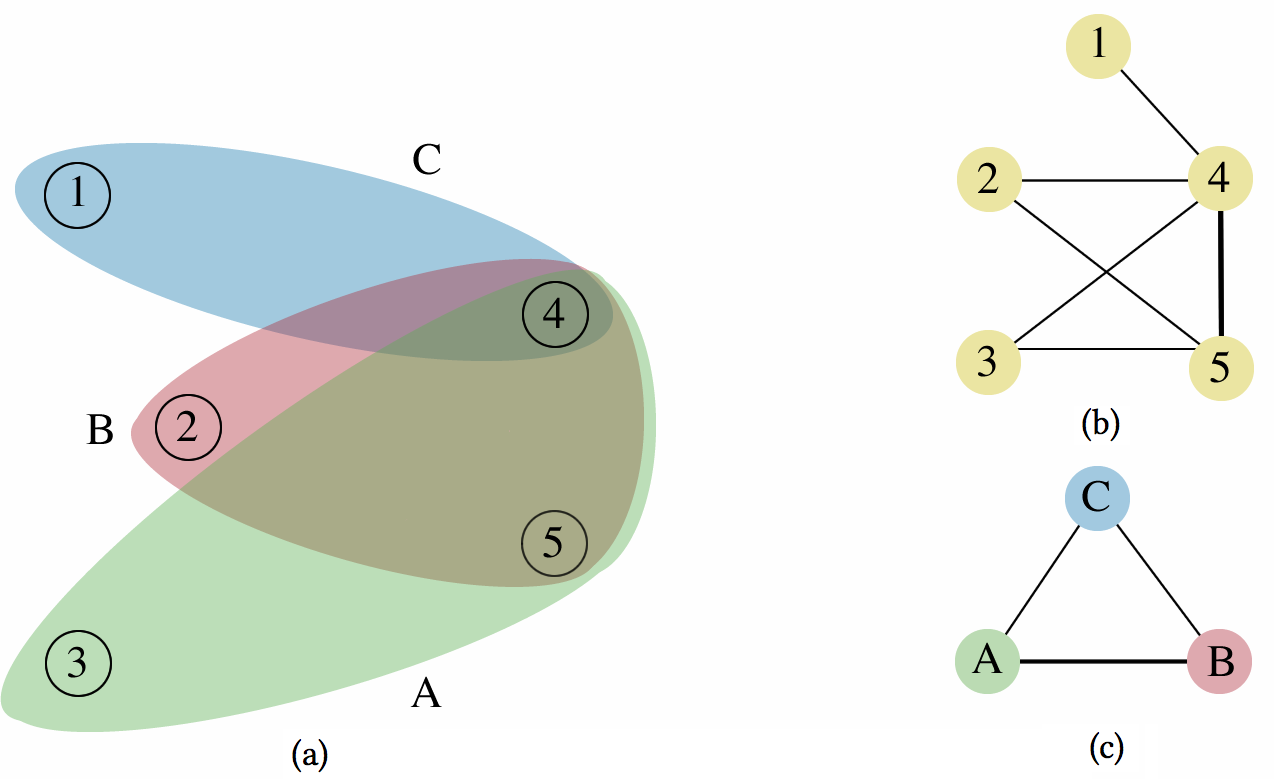
\includegraphics[scale=0.28]{imgs/hypergraph.png}
\end{center}
\caption[Hypergraph and network projections]{Figure (a) is a hypergraph containing five nodes and three affiliations. Network (b) is the affiliation projection of hypergraph (a). Network (c) is the node projection of hypergraph (a).}
\label{hypergraph}
\end{figure}

\subsubsection*{Networks}

A hypergraph can be projected into two networks: the first is a \emph{node projection} and the second is an \emph{affiliation projection}. The projections are represented as networks and therefore we use the term `network' and `projection' interchangeably. These projections are useful for assessing overlapping and interlocking directorates of firms, which will be assessed throughout the chapter.

\paragraph{Node projection.}

A hypergraph can be projected on the node set $N$. A node projection of the hypergraph $\Gamma$ is denoted by $g_N$, which refers to the set of relationships $g_N = \{ij \, \mid \, j \in \overline{\Gamma}_{i} \mbox{ and } i \neq j \}$, where $ij$ is an \emph{undirected link} between nodes $i$ and $j$, such that $ij = ji$, therefore if $ij \in g_{N}$ then $ji \in g_{N}$. The node network from the hypergraph in Figure~\ref{hypergraph} (a) can be seen in Figure~\ref{hypergraph} (b).

\paragraph{Affiliation projection.}

Furthermore, a hypergraph can be projected into an affiliation projection on the set of affiliations, $\Gamma$. An affiliation network of the hypergraph $\Gamma$ is denoted by $G_{\Gamma}$, which refers to a set of reciprocated \emph{arcs} $G_{\Gamma} = \{ HK \, \mid \, K \in \mathcal{E}_{H} \mbox{ and } H \in \Gamma \}$. The affiliation network from the hypergraph in Figure~\ref{hypergraph} (a) can be seen in Figure~\ref{hypergraph} (c).

The links between the nodes the in the node projection of a hypergraph can have a weight determined by the number of mutual affiliations between the nodes. Moreover, the arcs in the affiliation projection can have a weight determined by the number of mutual nodes between the affiliations. Formally, with respect to the node projection, the weight on an a link between a pair of nodes $i,j \in N$ is given by
\begin{equation} \label{eq:nodeweight}
\omega_{ij}(\Gamma) = | \overline{\Gamma}_{i} \cap \overline{\Gamma}_{j} | .
\end{equation}
Also, with respect to the affiliation projection, the weight on an arc from affiliation $H \in \Gamma$ to another affiliation $K \in \Gamma$ is given by
\begin{equation} \label{eq:affweight}
\omega_{HK}(\Gamma) = | H \cap K | .
\end{equation}
If $\omega_{ij}(g_{N}) = 0$ then there does not exist a weighted undirected link between nodes $i$ and $j$. Likewise, if $\omega_{HK}(G_{\Gamma}) = 0$ then there exists no weighted arc from $H$ to $K$.

\subsection{Degree-based centrality measures in affiliation situations} 
\label{degreecentralities}

We provide a centrality measure for nodes and affiliations within the context of a hypergraph to be used in the analysis of empirical situations. The measure is directly related to the dependence of the affiliation on the individual node and the value of the affiliation(s) that the node is a member of. We use this to measure the influence of individual nodes and affiliations within a hypergraph.

Within this chapter we define `influence' as the ability for agents to control resources; which has particular importance with regard to directorate hypergraphs whereby the influence of a director is given by the voting rights of the director and the size of the firm(s) that they are members of. Indeed, having proportionally more voting rights to the decisions of a firm and/or being a board member of a highly valued firm will increase a directors influence on the resources that the firm owns. From this we can derive the external influence of an affiliation or firm, which refers to the total amount of resources that it can potentially control beyond itself. We define the influence of an individual or affiliation---given by the $\sigma$-score---in its most general form as a centrality measure on a hypergraph.
\begin{definition}
Let $N = \{ 1, \ldots ,n \}$ be a given set of nodes. A \textbf{centrality measure} on $N$ is a function $\varphi \colon N \times \mathbb{H}^N \to \mathbb{R}^N$.
\end{definition}
A centrality measure on $N$ is a function that for every affiliation situation represented by a hypergraph $\Gamma \subset 2^N$ assigns to every individual node $i \in N$ a real number $\varphi_i ( \Gamma )$ representing the importance of $i$ in $\Gamma$. Ideally the measure should correctly represent the importance of an individual in the corporate situation represented by $\Gamma$.

There exists no specific measure of centrality for hypergraphs; most measures are either derived from the degree of the node or derived from the paths and walks that a node lies on. We specifically focus on degree-based measures, elaborating on the standard degree measure, the generalised $\beta$-measure, and influence.

\subsubsection*{Standard degree measure}

The \emph{standard degree measure} is the centrality measure $\delta \colon N \times \mathbb{H}^N \to \mathbb{R}^N$, which for every node $i \in N$ is defined by
\begin{equation}
\delta_i (\Gamma ) = \left| \overline{\Gamma}_i \right| .
\end{equation}
For general hypergraphs the sum of the standard degree across all nodes is computed as
\begin{equation}
\sum_{i \in N} \delta_i (\Gamma ) = \sum_{H \in \Gamma} | H | \, ( \, | H | - 1) - \sum_{H,H' \in \Gamma} | H \cap H' | \cdot \frac{| H \cap H' | - 1}{2} .
\end{equation}
For hypergraphs where $| H | = 2$ for all $H \in \Gamma$, this simplifies to $\sum_{i \in N} \delta_i (\Gamma ) = \sum_{H \in \Gamma} | H | \, ( \, | H | - 1) = 2 \, | \Gamma |$. These are networks.

If $\Gamma$ is projected as a node network, $g_N$, the standard degree measure simplifies to the standard degree concept defined and used in network analysis given by
\begin{equation}
\delta_i (\Gamma ) = d_i (g_N ) = | \, \{ j \in N \mid \, j  \in \Gamma_{i} \mbox{ where } j \neq i \}  \, |.
\end{equation}
Likewise, for node projected hypergraphs where $| H | = 2$ for all $H \in \Gamma$ in the initial hypergraph, $\sum_{i \in N} d_i (g_{N}) = 2 \, | \Gamma |$.

Finally, we denote the degree of an affiliation, $H \in \Gamma$, in the affiliation projection of $\Gamma$ as $\delta_{H}(G_{\Gamma}) = | \mathcal{E}_{H} |$, or simply as $\delta_{H}$.

\subsection{A hypergraph $\beta$-measure}

The \emph{hypergraph} $\beta$-\emph{measure} is the centrality measure $\beta \colon N \times \mathbb{H}^N \to \mathbb{R}^N$ given by
\begin{equation}
\beta_i (\Gamma ) = \sum_{j \in \overline{\Gamma}_i} \frac{1}{\left| \, \overline{\Gamma}_j \right|}
\end{equation}
In the case that $\Gamma$ is a network on $N$ this simplifies to
\begin{equation}
\beta_i (g_{N}) = \sum_{j \in \overline{\Gamma}_i} \frac{1}{d_j (\Gamma )} \equiv \beta_i (\Gamma ) .
\end{equation}
which is indeed equivalent to the original formulation of the $\beta$-measure for networks by van den Brink and Gilles (1994). The $\beta$-measure is a measure of dominance whereby some node, $i$, dominates another, $j$, if $ij \in g_{N}$ or $\Gamma_{i} \cap \Gamma_{j} \neq \varnothing$. The total dominance distributed across the node set of the hypergraph is given by the total number of nodes that participate in at least one affiliation. We note this formally as
\begin{equation}
\sum_{i \in N} \beta_{i}(\Gamma) = | ~ \{ i \in N ~ | ~ \Gamma_{i} \neq \varnothing \} ~ | .
\end{equation}
The standard $\beta$-measure can be supported as a Shapley value of a corresponding TU-game describing the power relations in an affiliation situation.\footnote{A \textbf{TU-game} or ``cooperative game with transferable utilities'' on the node set $N$ is a function $v \colon 2^N \to \mathbb{R}$ such that $v( \varnothing )=0$. It describes the values that can be generated by groups of nodes in the affiliation situation under consideration. The \emph{Shapley value} of a TU-game $v$ is defined as $\phi_i (v) = \sum_{S \colon i \in S} \frac{\Delta_v (S)}{|S|}$, where $\Delta_v (S) = \sum{T \subset S} (-1)^{|S|-|T|} v(T)$ is the \emph{Harsanyi dividend} of the coalition $S$ in the game $v$.}
\begin{theorem}
Let $\Gamma$ be some affiliation situation on node set $N$. We define $V_{\Gamma} \colon 2^N \to \mathbb{R}$ as the TU-game given by
\begin{equation}
v_{\Gamma} (S) = \left| \, \cup_{j \in S} \overline{\Gamma}_j \, \right| .
\end{equation}
Then the Shapley value of $V_{\Gamma}$ coincides with the $\beta$-measure for $\Gamma \colon$
\begin{equation}
\phi_i \left( V_{\Gamma} \right) = \beta_i (\Gamma ) .
\end{equation}
\end{theorem}
\begin{proof}
This proof follows the outline of the proof of a corresponding result for the $\beta$-measure for networks given in Gilles (2010).
\\
Let $\Gamma \subset 2^N$ be some affiliation situation on $N$. For every node $i \in N$ we define a TU-game $w_i \colon 2^N \to \mathbb{R}$ by
\begin{equation}
w_i (S) = \left\{
\begin{array}{ll}
1 & \mbox{if } S \cap \overline{\Gamma}_i \neq \varnothing \\
0 & \mbox{otherwise}
\end{array} \right. .
\end{equation}
Then it is clear that for every $S \subset N$
\begin{equation}
V_{\Gamma} (S) = \sum_{i \in N} w_i (S) \quad \mbox{or} \quad V_{\Gamma} = \sum_{i \in N} w_i
\end{equation}
and, therefore, by additivity of the Shapley value it holds that for every $j \in N \colon$
\begin{equation}
\phi_j \left( V_{\Gamma} \right) = \sum_{i \in N} \phi_j \left( w_i \right) .
\end{equation}
We can determine that the Harsanyi dividends for $w_i$ are given by $\Delta_{w_i} (S) = (-1)^{|S|+1}$. Therefore,
\begin{equation}
\phi_j (w_i) = \sum_{S \subset N \colon j \in S} \frac{\Delta_{w_i} (S)}{|S|} = \sum_{S \subset \overline{\Gamma}_i \colon j \in S} \frac{(-1)^{|S|+1}}{|S|} .
\end{equation}
Hence, for every $j \in N \colon$
\begin{align*}
\phi_j \left( V_{\Gamma} \right) & = \sum_{i \in N} \phi_j (w_i) = \sum_{i \in N} \, \sum_{S \subset \overline{\Gamma}_i \colon j \in S} \frac{(-1)^{|S|+1}}{|S|} \\[1ex]
& = \sum_{i \in \overline{\Gamma}_j} \, \sum_{S \subset \overline{\Gamma}_i \setminus \{ i \} } \frac{(-1)^{|S|}}{|S|+1} \\[1ex]
& = \sum_{i \in \overline{\Gamma}_j} \, \sum^{D_i-1}_{t=0} \binom{D_i-1}{t} \, \frac{(-1)^t}{t+1}
\end{align*}
where we use the shorthand $D_i = \left| \overline{\Gamma}_i \right|$. Now,
\begin{align*}
\sum^{D_i-1}_{t=0} \binom{D_i-1}{t} \, \frac{(-1)^t}{t+1} & = \frac{-1}{D_i} \, \left[ \, \sum^{D_i}_{t=1} \binom{D_i}{t} \cdot (-1)^t \, \right] = \\[1ex]
& = \frac{-1}{D_i} \, \left[ \, \sum^{D_i}_{t=0} \binom{D_i}{t} \cdot (-1)^t -1 \, \right] = \\[1ex]
& = \frac{-1}{D_i} \, \left[ \, (1-1)^{D_i} -1 \, \right] = \frac{1}{D_i} .
\end{align*}
Therefore,
\[
\phi_j \left( V_{\Gamma} \right) = \sum_{i \in \overline{\Gamma}_j} \frac{1}{D_i} = \sum_{i \in \overline{\Gamma}_j} \frac{1}{\left| \overline{\Gamma}_i \right|} = \beta_j (\Gamma )
\]
This shows the assertion.
\end{proof}

\paragraph{Generalised $\beta$-measure.}

The $\beta$-measure can be generalised such that there can exist weights on the relations between the nodes. This is for specific application to weighted directed or undirected networks, however we can derive the $\beta$-scores of nodes given that there can exist weighted relations between nodes in the node projection of the hypergraph.

Let $\Gamma$ be a hypergraph on node set $N$, where $i,j \in N$, the \emph{generalised $\beta$-measure}, denoted by $\beta^{\star}_{i}(\Gamma)$ for some node $i$, is given by
\begin{equation}
\beta^{\star}_{i}(\Gamma) = \sum_{j \in \overline{\Gamma}_{i}} \frac{\omega_{ij}(g_{N})}{W_{j}(\Gamma)} ,
\end{equation}
where $\omega_{ij}(g_{N}) = | \Gamma_{i} \cap \Gamma_{j} |$, as in Equation~\ref{eq:nodeweight}, and $W_{i}(\Gamma) = \sum_{i \in \overline{\Gamma}_{j}} \omega_{ij}(\Gamma)$. The generalised $\beta$-measure distributes the dominance weight of a node proportional to the weights of the relations on which node $j$ is dominated. These weights emerge, as noted above, in the node projection of the hypergraph. A non-weighted network is equivalent to the weighted network with
\[
\omega_{ij}(g_{N} ) = \left\{
\begin{array}{ll}
1 & \mbox{if } \Gamma_{i} \cap \Gamma_{j}  \\
0 & \mbox{otherwise .}
\end{array} \right.
\]
But then $W_{j}(\Gamma) = d_{j}(\Gamma)$ for all $j \in N$ and $\omega_{ij}(\Gamma) = \omega_{ij}(g) \in \{0,1\}$, so $\beta^{\star}_{i}(\Gamma) = \beta_{i}(\Gamma)$. Thus, the generalised $\beta$-measure is indeed a generalisation of the $\beta$-measure.

With respect to the set of affiliations, we can measure their $\beta$-score in much the same way as with the generalised $\beta$-measure for the node set. Let $\Gamma$ be a hypergraph where $H, K \in \Gamma$ are affiliations and let
\begin{equation}
W_{K}(\Gamma) = \sum_{H \in \mathcal{E}_{K}} \omega_{HK}(G_{\Gamma}) ,
\end{equation}
where $\omega_{HK}(G_{\Gamma})$ is given by Equation~\ref{eq:affweight}. The generalised $\beta$-measure for affiliations is now given by
\begin{equation}
\beta^{\star}_{H}(\Gamma) = \sum_{K \in \mathcal{E}_{H}} \frac{\omega_{HK}(G_{\Gamma})}{W_{K}(\Gamma)} .
\end{equation}
Much like above, this leads to the property that $\sum_{H \in \Gamma} \beta^{\star}_{H} (\Gamma) = | ~ \{ H \in \Gamma ~ | ~ H \neq \varnothing \} ~ |$.

\paragraph{Axiomatisation of the generalised $\beta$-measure.}

The generalised $\beta$-measure can be characterised through the use of four axioms. We present these axioms on an arbitrary relational power measure $f : \mathbb{H}^{N} \rightarrow \mathbb{R}^{N}$, where any hypergraph structure, $\Gamma$, can be drawn from $\mathbb{H}^{N}$, that uniquely determine the generalised $\beta$-measure. These axioms are as follows.

\begin{axiom}[Weighted dominance normalisation] \label{ax:1}
For every $\Gamma \in \mathbb{H}^{N}$ it holds that
\[
\sum_{i \in N} f_{i}(\omega) = | ~ \{ j \in N ~ | ~ \lambda_{\omega}(j) > 0 \} ~ |
\]
\end{axiom}

\begin{axiom}[Weighted dummy node property] \label{ax:2}
For every $\Gamma \in \mathbb{H}^{N}$ and every $i \in N$ with $\Gamma_{i} = \varnothing$ it holds that $f_{i}(\omega) = 0$.
\end{axiom}

\begin{axiom}[Weight proportionality] \label{ax:3}
For every $\Gamma \in \mathbb{H}^{N}$ and every pair $i,j \in N$ for which there is a constant $c_{i,j} \in \mathbb{R}$ such that $\omega(i,h) = c_{i,j} \cdot \omega(j,h)$ for every $h \in N$ it holds that
\begin{equation}
f_{i}(\omega) = c_{i,j} \cdot f_{j}(\omega) ~ .
\end{equation}
\end{axiom}

To state the fourth axiom we introduce a partition of a hypergraph $\Gamma$ as a collection of hypergraphs $\mathcal{G} = \{\Gamma_{1}, \ldots, \Gamma_{m}\}$ such that $\sum_{\ell = 1}^{m} \omega_{ij}^{\ell} = \omega_{ij}$ for every $ij \in g_{N}$.


\begin{axiom}[Additivity over weighted independent partitions] \label{ax:4}
For every $\Gamma \in \mathbb{H}^{N}$ and independent partition $\mathcal{G}$ of $\Gamma$ it holds that
\begin{equation}
f(\omega) = \sum_{\omega_{k} \in \mathcal{G}} f(\omega_{k})
\end{equation}
\end{axiom}

The generalised $\beta$-measure satisfies these four axioms.

\subsection{A standard $\sigma$-score}

An alternative centrality measure is the \emph{$\sigma$-score} defined as the centrality measure $\sigma \colon N \times \mathbb{H}^N \to \mathbb{R}^N$ with for every node $i \in N \colon$
\begin{equation}
\sigma_i (\Gamma ) = \sum_{H \in \Gamma_i} \frac{1}{|H|}
\end{equation}
\begin{proposition} \label{prop:SG-degree}
Let $\Gamma$ be a hypergraph. If $| H | = 2$ for all $H \in \Gamma$, the $\sigma$-score becomes
\begin{equation}
\sigma_i (\Gamma ) = \tfrac{1}{2} \delta_i ( \Gamma ) ,
\end{equation}
meaning that $\sigma_{i}(G_{\Gamma}) = \tfrac{1}{2} d_{i} (G_{\Gamma})$ in the affiliation projection.
\end{proposition}
Due to Proposition~\ref{prop:SG-degree} the $\sigma$-score is to be viewed as a degree-based measure. In fact, in comparison with the standard degree measure, it is an alternative generalisation of the degree concept used in network analysis to the realm of hypergraphs or affiliation situations. Further still, we will show that the \emph{weighted $\sigma$-score} is a further generalisation of the generalised $\beta$-measure.

The normalisation of the $\sigma$-score on the node set $N$ of general hypergraphs is different from the normalisation of the degree measure and the $\beta$-measure. This normalisation is given by
\begin{equation} \label{eq:sigmanorm}
\sigma_{N} = \sum_{i \in N} \sigma_i (\Gamma ) = | \Gamma | .
\end{equation}
Equation~\ref{eq:sigmanorm} clearly indicates that the $\sigma$-score is a normalised degree measure that normalises to the number of affiliations in hypergraph $\Gamma$.

Regardless of both measures being degree-based Example~\ref{comparedegree} shows that different centrality measures can provide substantially different outcomes of relative node centrality. Specifically we note that the relative centrality of nodes changes with the measure that is given, with node $1$ becoming relatively more important surpassing nodes $2$ and $3$ when considering the $\sigma$-score.

\begin{example} \label{comparedegree}
Consider the hypergraph, $\Gamma $, on node set $N = \{ 1, 2, 3, 4, 5\}$ shown in Figure~\ref{hypergraph} (a). The standard degree measure on all nodes is given by the vector, $\delta(\Gamma ) = ( 1, 2, 2, 4, 3)$, the generalised $\beta$-measure on all nodes is given by the vector, $\beta^{\star}(\Gamma) = ( \frac{1}{5}, \frac{9}{20}, \frac{9}{20}, \frac{5}{2}, \frac{7}{5} )$, and the $\sigma$-score on all nodes is given by the vector, $\sigma(\Gamma ) = ( \frac{1}{2} , \frac{1}{3}, \frac{1}{3}, \frac{7}{6}, \frac{2}{3} )$.
% Add the standard beta-score
\end{example}

The substantial differences mean that both measures concern different traits of node connectivity that influence the importance of a node. Specifically, the $\sigma$-score is fundamentally tied to the quantity and context of affiliations that a node is embedded, and is thus more attuned to the affiliations of the hypergraph. On the other hand the standard degree and $\beta$-measures is only concerned with the resulting network structure from the existence of affiliations and each nodes' membership to these affiliations \footnote{We highlight a restriction of the $\sigma$-score by noting that, unlike the standard degree measure, it cannot be used with respect to general projections of a hypergraph to a node network. Indeed, whereas the standard degree measure has direct application to a node network, this is only true with the $\sigma$-score where $| H | = 2$ for all $H \in \Gamma$.}.

\paragraph{Weighted $\sigma$-score.}

The $\sigma$-score can be generalised for use in weighted hypergraphs defined by the triple $\Gamma' = (N, \Gamma, \mathbf{v})$. The generalised $\sigma$-score is defined as the centrality measure $\sigma' : N \times \mathbb{L}^{N} \rightarrow \mathbb{R}^{N}$, with for every node $i \in N$:
\begin{equation}
\sigma'_{i}(\Gamma' ) = \sum_{H \in \Gamma_{i}' } \frac{\nu_{H}}{| H |} .
\end{equation}
The normalisation of the weighted $\sigma$-score subsequently becomes
\begin{equation} \label{sigmanorm}
\sum_{i \in N} \sigma'_{i}(\Gamma' ) = \sum_{H \in \Gamma' } \nu_{H} = V(\Gamma').
\end{equation}
\begin{example} \label{weightedSG}
Let the hypergraph on node set $N = \{ 1, 2, 3, 4, 5\}$ shown in Figure~\ref{hypergraph} (a) be a weighted hypergraph $\Gamma'$ where $\nu_{A} = 21$, $\nu_{B} = 15$, and $\nu_{C} = 8$, such that $V(\Gamma') = \sum_{H \in \Gamma'} \nu_{H} = 44$. The normalised weighted $\sigma$-score for all nodes is given by the vector, $\sigma'(\Gamma' ) = ( \frac{1}{11}, \frac{5}{44}, \frac{7}{44}, \frac{4}{11}, \frac{3}{11} )$.
\end{example}
Example~\ref{weightedSG} shows that the weight of an affiliation can have an impact on the centrality of a node. Specifically node $1$ now becomes relatively less important than both nodes $2$ and $3$, and there is a differential that emerges between nodes $2$ and $3$.

Where the value of an affiliation may matter, as in directorate networks, the initial $\sigma$-score bias the centrality of nodes. Specifically, nodes that are members of an affiliation with a small population (such as in the case with node $1$) may have a large centrality regardless of the value of the affiliation that they are members of. Further biases can emerge in the other direction whereby nodes that are members of affiliations with a large population could have a downward bias on their centrality.

\medskip \noindent To this point the $\sigma$-score has been applied to nodes only. This is extended to affiliations such that the $\sigma$-score of an affiliation within a weighted hypergraph is given by
\begin{equation}
\sigma_{H}(\Gamma') = \left( \sum_{K \in \mathcal{E}_{H}} \nu_{K} \cdot \frac{| H \cap K |}{| K |} \right) + \nu_{H},
\end{equation}
which simplifies to
\begin{equation}
\sigma'_{H}(\Gamma' ) = \sum_{i \in H} \sigma'_{i}(\Gamma ' ).
\end{equation}

\begin{example} \label{ex:influence}
Consider the weighted hypergraph, $\Gamma '$, on node set $N = \{ 1, 2, 3, 4, 5\}$ from Example~\ref{weightedSG} where $\nu_{A}(\Gamma' ) = 21$, $\nu_{B}(\Gamma' ) = 15$, $\nu_{C}(\Gamma' ) = 8$, and $V (\Gamma' ) = 44$. The normalised $\sigma$-score of each affiliation is given by the vector, $\Sigma(\Gamma' ) = ( \frac{35}{44}, \frac{3}{4}, \frac{5}{11} )$.

Furthermore we also highlight the relationship between the $\sigma$-score of the affiliations and the $\sigma$-scores of the individual nodes. From Example~\ref{weightedSG} we find that $A = \{3,4,5\}$ and $\sigma_{3}(\Gamma') + \sigma_{4}(\Gamma') + \sigma_{5}(\Gamma') = \frac{7}{44} + \frac{4}{11} + \frac{3}{11} = \frac{35}{44} \equiv \Sigma_{A}(\Gamma')$; $B = \{2,4,5\}$ and $\sigma_{2}(\Gamma') + \sigma_{4}(\Gamma') + \sigma_{5}(\Gamma') = \frac{5}{44} + \frac{4}{11} + \frac{3}{11} = \frac{3}{4} \equiv \Sigma_{B}(\Gamma')$; and finally $C = \{1,4\}$ and $\sigma_{1}(\Gamma') + \sigma_{4}(\Gamma') = \frac{1}{11} + \frac{4}{11} = \frac{5}{11} \equiv \Sigma_{C}(\Gamma')$.
\end{example}

Note that there does not always exist a relative relationship between the $\sigma$-score of an affiliation and its value in the weighted hypergraph. Moreover, this phenomenon may also not exist for the so-called external influence of the affiliation\footnote{The external influence of an affiliation only takes into consideration the influence that the affiliation has beyond itself.}. The \emph{external influence} of some affiliation $H \in \Gamma$ is given by
\begin{equation}
\sigma^{\star}_{H}(\Gamma' ) = \sigma'_{H}(\Gamma' ) - \nu_{H}
\end{equation}
In the case of Example~\ref{ex:influence} affiliation $B$ has the highest external influence even though affiliation $A$ has the highest value.

\begin{property} \label{prop:norm}
Let $\Gamma$ be a hypergraph on node set $N$ and $G_{\Gamma}$ be the affiliation projection of $\Gamma$.
\begin{abet}
\item $\sum_{i \in N} \sigma_{i}(\Gamma) = | ~ \{ H \in \Gamma~|~H \neq \varnothing \} ~ | = | \Gamma |$.

By extension, $\sum_{i \in N} \sigma_{i}(\Gamma') = \sum_{H \in \Gamma'} \nu_{H}$.

\item $\sum_{H \in \Gamma} \sigma_{H}(\Gamma) = | \Gamma | + \sum_{H \in \Gamma} \left( \sum_{K \in \mathcal{E}_{H}} \frac{| H \cap K |}{|K|} \right)$.

By extension, $\sigma_{\Gamma}(\Gamma') = \sum_{H \in \Gamma} \sigma_{H}(\Gamma') = V(\Gamma') + \sum_{H \in \Gamma} \left( \sum_{K \in \mathcal{E}_{H}} \nu_{K} \cdot \frac{| H \cap K |}{|K|} \right) $.

% This simplifies to $\sigma_{\Gamma}(\Gamma) = 2 | \Gamma |$ and $\sigma_{\Gamma}(\Gamma') = 2 V(\Gamma')$ if $| \Gamma_{i} | > 1$ and $\nexists ~ \mathcal{H} \subseteq \Gamma'$ such that $\cup \mathcal{H} = \varnothing$ and $| H | > 1$ for all $H \in \mathcal{H}$.
\end{abet}
\end{property}

In non-weighted hypergraphs, $\Gamma$, $\nu_{H} = 1$ for all $H \in \Gamma$. The weighted $\sigma$-score is equivalent to the $\sigma$-score when standardising all affiliation weights to 1, suggesting that the weighted $\sigma$-score is a generalised version of the $\sigma$-score.

\subsubsection*{Equivalence between the $\sigma$-score and the $\beta$-measure}

When considering the affiliation projection of the non-weighted hypergraph there emerges an equivalence between the $\sigma$-score and the $\beta$-measure of affiliations. We note that the $\beta$-score of some $H \in \Gamma$ in the affiliation projection $G_{\Gamma}$ is given by
\begin{equation}
\beta^{\star}_{H}(G_{\Gamma}) = \sum_{K \in \mathcal{E}_{H}} \frac{\omega_{HK}(G_{\Gamma})}{W_{K}(G_{\Gamma})} ,
\end{equation}
where $W_{K}(G_{\Gamma}) = \sum_{H \in \mathcal{E}_{K}} \omega_{HK} (G_{\Gamma})$.

The $\sigma$-score of an affiliation in the affiliation projection of a non-weighted hypergraph is given by
\begin{equation}
\sigma_{H}(G_{\Gamma}) = \left( \sum_{K \in \mathcal{E}_{H}} \omega_{HK}(G_{\Gamma}) \right) + 1
\end{equation}
Therefore, $\beta^{\star}_{H}(\Gamma) = \sigma_{H}(\Gamma) - 1$ if $W_{K}(G_{\Gamma}) = 1$ for all $K \in \mathcal{E}_{H}$. Example~\ref{ex:equiv} highlights this equivalence between the generalised $\beta$-measure and $\sigma$-score.

\begin{example} \label{ex:equiv}
Consider the hypergraph $\Gamma$ in Figure~\ref{hypergraph}(a) and the affiliation projection, $G_{\Gamma}$, in Figure~\ref{hypergraph}(c). The weights attached to the arcs were calculated in Example~\ref{comparedegree}; from these the generalised $\beta$-measure and $\sigma$-score for each affiliation can be calculated.

$W_{A}(G_{\Gamma}) = W_{B}(G_{\Gamma}) = W_{C}(G_{\Gamma}) = 1$ meaning that $\beta^{\star}_{A}(G_{\Gamma}) =\beta^{\star}_{B}(G_{\Gamma}) = \frac{7}{6}$ and $\beta^{\star}_{C}(G_{\Gamma}) = \frac{2}{3}$. Likewise, $\sigma_{A}(G_{\Gamma}) = \sigma_{B}(G_{\Gamma}) = \frac{13}{6}$ and $\sigma_{C}(G_{\Gamma}) = \frac{5}{3}$. Therefore, $\beta_{H}(G_{\Gamma}) = \sigma_{H}(G_{\Gamma}) - 1$ for all $H \in \Gamma$.
\end{example}

\section{Hypergraphs with aspects} \label{Theory:Elites}

We introduce the notion of \emph{aspectual hypergraphs}, i.e., hypergraphs with aspects. In general an \emph{aspect} refers to a set of nodes, or affiliations, categorised by a certain observable or well-defined characteristic. Specifically in our case we define an aspect as a certain division of labour that an affiliation specialises in; it is therefore comparable to an industry within which a set of firms operates in. The aspect(s) to which each individual node participates is derived from the set of affiliations that they are members of and the aspects that the affiliations are subsequently embedded in.

\subsection{Aspectual hypergraphs}

\paragraph{Aspectual hypergraphs.}

The set of \emph{aspects} in a hypergraph is given by
\begin{equation}
\mathcal{A} = \{ A ~ | ~ A \subseteq \Gamma \mbox{ and } A \cap A' = \varnothing \mbox{ for any } A' \subseteq \Gamma \} ,
\end{equation}
where $| \mathcal{A} | = a$. Subsequently, an \emph{aspectual hypergraph} is defined by the triple $\Gamma_{\mathcal{A}} = (\Gamma, N, \mathcal{A})$ and, for completeness, a \emph{weighted aspectual hypergraph} is defined by the quadruple $\Gamma'_{\mathcal{A}}= (\Gamma, N, \mathbf{v}, \mathcal{A})$.

We let $\mathcal{A}_{H} = \{ A \in \mathcal{A} \, \mid \, H \in A\}$ and $\mathcal{A}_{H} \neq \varnothing$ for all $H \in \Gamma$. We highlight the restriction such that $| \mathcal{A}_{H} | = 1$ for all $H \in \Gamma$, which provides disjointed partitions of affiliations into aspectual spaces\footnote{However the restriction could be weakened for future work.}.

Nodes also operate in at least one aspect as a consequence of being a member of more than one affiliation. The set of aspects that some $i \in N$ operates in is given similarly given by $\mathcal{A}_{i} = \{ A \in \mathcal{A}_{H} \, \mid \, i \in H \}$. The player set of a given aspect $A \in \mathcal{A}$ is given as $N(A) = \{ i \in N \, \mid \, i \in H \text{ and } \mathcal{A}_{H} = A \}$.

\subsubsection*{Aspectual distance}

Aspects can overlap with respect to their node set. The degree in which a pair of aspects overlap is determined by the number of nodes associated with both aspects.

\begin{definition}
The \textbf{distance} between a pair of aspects, $A$ and $A'$, is given by:
\begin{equation}
\mbox{dist}(A, A',\Gamma_{\mathcal{A}}) = 1 - \frac{| N(A) \cap N(A') |}{| N(A) |} ~ ,
\end{equation}
where $\mbox{dist}(A, A',\Gamma_{\mathcal{A}}) \in [0,1]$.
\end{definition}

If $N(A) \subseteq N(A')$, then $\mbox{dist}(A, A', \Gamma_{\mathcal{A}}) = 0$; therefore, the more overlapping a pair of aspects then the closer to $0$ the distance between the aspects will be. Note, $\mbox{dist}(A, A',\Gamma_{\mathcal{A}}) = \mbox{dist}(A, A',\Gamma_{\mathcal{A}}) \iff | N(A) | = | N(A') |$.

The overlap of aspects provides an indicator for how many bridge relations are contained between the aspects. As $\mbox{dist}(A, A',\Gamma_{\mathcal{A}}) \rightarrow 1$ then fewer bridge relations exist from aspect $A$ to aspect $A'$, meaning that if $\mbox{dist}(A, A',\Gamma_{\mathcal{A}}) = 1$ no bridges exist. If there are only a few nodes that intersect between aspects there must exist more power in those nodes to bridge relations between aspects. Conversely, if there are relatively many nodes in the intersection between the aspects, then there will be limited scope for brokerage between the aspects. Power to broker relations and information between aspects is centralised in the intersection between aspects.

\begin{example} \label{ex:dist}
Let the hypergraph on node set $N = \{1,2,3,4,5\}$ from Figure~\ref{hypergraph}(a) be an aspectual hypergraph $\Gamma_{\mathcal{A}}$. This hypergraph has an aspect set given by $\mathcal{A} = \{A_{1}, A_{2} \}$, where $A_{1} = \{A,B\}$ and $A_{2} = \{C\}$. Given this we calculate the asymmetrical distances to be $\mbox{dist}(A_{1}, A_{2}, \Gamma_{\mathcal{A}}) = \frac{1}{4}$ and $\mbox{dist}(A_{2}, A_{1}, \Gamma_{\mathcal{A}}) = \frac{1}{2}$. Node $4$ is the single broker between the two aspects.
\end{example}

The notion of aspectual bridging can be complemented with the `correlation' between aspects. Indeed, although power is centralised within the intersection of aspects---the bridging relations---they will be more valuable if the aspects are highly correlated with, and therefore complimenting of, each other.

\subsubsection*{Aspectual correlation}

Aspects can be alike such that fluctuations in their structure and value can be correlated with each other. The relationship to which aspects are correlated should therefore be considered in the context that they are analysed. Within this chapter we consider the correlation between aspects to be a function of how the value of an aspect and its affiliations change over time.

We let the value of some aspect, $A \in \mathcal{A}$, in some time period $t \in \{1,\ldots,T\}$ be given by
\begin{equation}
\mu(A_{t}) = \sum_{H \in A} \nu_{H}(\Gamma'_{\mathcal{A}} ) .
\end{equation}
The likeness between a pair of assets is computed in the conventional fashion through the calculation of the standard deviation and covariance of the values of each pair of aspects. Specifically, let the standard deviation of some aspect, $A$, be calculated as
\begin{equation}
\lambda(A) = \sqrt{\frac{\sum_{t=1}^{T} \left[ \mu(A_{t}) - \overline{\mu}(A) \right]^{2}}{T}} ~ ,
\end{equation}
where
\begin{equation}
\overline{\mu}(A) = \frac{\sum_{t=1}^{T} \mu(A_{t})}{T} ~ ,
\end{equation}
and $T > 0$ is the number of time periods. From this, the covariance of two aspects, $A,A' \in \mathcal{A}$, is calculated by:
\begin{equation}
Cov(A,A') = \frac{\sum_{t=1}^{T} \left[ \mu(A_{t}) - \overline{\mu}(A) \right] \cdot \left[ \mu(A'_{t}) - \overline{\mu}(A') \right]}{T} ~ .
\end{equation}
Thus, the \emph{aspectual correlation} between the two aspects is given as:
\begin{equation}
r(A,A',\Gamma'_{\mathcal{A}}) = \abs{ ~ \frac{Cov(A,A')}{\lambda(A) \cdot \lambda(A')} ~ } ~ ,
\end{equation}
such that $r(A,A',\Gamma'_{\mathcal{A}}) \in [0,1]$, since the absolute value of the correlation co-efficient is used. As $r(A,A',\Gamma'_{\mathcal{A}}) \rightarrow 1$ the relationship between aspects increases; a change in the value of one aspect is reflected in a change in the value of another. The absolute value of the correlation is used because, regardless of whether the relationship is positive or negative the relationship can be used to assess the connectivity of the aspects.

The relationship between a pair of aspects is therefore informed by the variance and covariance of the pairs values. This is a time-dependent measure, meaning that multiple time periods are required to provide a meaningful calculation. The calculation suggests that only the changes in the values over time are considered when measuring the relationship between aspects over time.

\medskip \noindent The importance of bridge relations between a pair of aspects is given by the product of the distance and correlation between them. Specifically, the importance of a bridge relation is formally given by:
\begin{equation}
\Lambda(A,A',\Gamma'_{\mathcal{A}}) = \mbox{dist}(A,A',\Gamma'_{\mathcal{A}}) \times r(A,A',\Gamma'_{\mathcal{A}}) ~ ,
\end{equation}
where $\Lambda(A,A',\Gamma'_{\mathcal{A}}) \in [0,1]$.

The power of the bridge relation is a scalar that corresponds to the benefit of operating within multiple aspects. The importance of bridge relations is therefore a positive function of the distance between the aspects that the relation is bridging and the correlation between those aspects.

If, for example, the distance between aspects increases with a given correlation, then the importance of bridge relations between the aspects will also increase. Conversely, if the correlation between aspects increases with a given distance, then the importance of the bridge relation increases.

\subsection{Elites and elite structures}

The importance of a node can be determined by both the structural attributes of the network--as shown by conventional measures of node centrality--and by the number of aspects that the node participates in. Section~\ref{degreecentralities} introduced and defined a number of measures of importance and centrality that were strictly increasing with the degree of the node or affiliation. Here we define a measure of importance that is not strictly increasing with the degree of the node. We consider the definition of an elite set of nodes as the collection of nodes that are embedded within all aspects of the network.

The set of elites, which can be derived from the aspectual hypergraph, is defined below.
\begin{definition}
Let $\Gamma_{\mathcal{A}}$ be an aspectual hypergraph on node set $N$ where affiliations are partitioned into aspects given by the class $\mathcal{A}$. The \textbf{elite set} is given by:
\begin{equation}
\mathcal{E} = \bigcap_{A \in \mathcal{A}} N(A) .
\end{equation}
Node $i \in N$ is an \textbf{elite} if and only if $i \in \mathcal{E} \subseteq N$, and therefore $\mathcal{A}_{i} = \mathcal{A}$.
\end{definition}
The notion of an elite is important because an elite will, by virtue of their direct links, have access to information regarding all aspects of the hypergraph. With respect to the application of directorate networks, a director who is a member of all aspects has direct access to information regarding all industries within the economy, and can therefore make more holistic and better informed decisions.

The measurement of elite is degree-based, but not strictly so. The relationship between the degree of a node in a hypergraph, i.e., the number of affiliations that it is a member of, and the likelihood that the node will be an elite is weakly monotonically increasing. Such a relationship can be seen in Appendix~\ref{A} whereby the probability of becoming an elite and the degree of the node is mapped. In Figure~\ref{RandSim1} the $x$-axes of the graphs show the proportion of affiliations that a node is a member of, and the $y$-axes show the probability of the node becoming an elite. We can see that it follows a typical binomial cumulative distribution function, which is characterised by the number of affiliations and the number of aspects for a given node degree.

\paragraph{Elite structure.}

The resulting set of elite nodes has a corresponding network structure. An \emph{elite structure} corresponds to the resulting network from the restricted set of nodes who are elite.

\begin{definition}
Let $\Gamma_{\mathcal{A}}$ be an aspectual hypergraph on node set $N$ and aspect class $\mathcal{A}$, where $g_{N}$ is the node projection of $\Gamma_{\mathcal{A}}$. The \textbf{elite structure} is given by the subnetwork $g_{\mathcal{E}}$, where
\begin{equation}
g_{\mathcal{E}} = \{ ij \in g_{N} ~ | ~ i,j \in \mathcal{E} \subseteq N \},
\end{equation}
\end{definition}

The elite structure is important with respect to directorate hypergraphs for two reasons. First, it highlights the proportion of directors, and their relations, that are embedded in multiple aspects of the economy. Second, if elites are embedded in multiple aspects together then they are more likely to have stronger relations and to share information between them; this structure is more likely to indicate a strong conduit of information dissemination. Arguably, centrality and brokerage in this network will be more reflective of power in the hypergraph.

%\paragraph{Eliteness:}
%
%The importance of an elite is reflected in their ability to access, use, broker, and potentially manipulate a diverse set of information. This notion of elites suggests that information is more diverse between aspects than within aspects; such a notion follows the fundamental assumption regarding \emph{structural holes} (Burt, 1992) and \emph{the strength of weak ties} (Granovetter, 1973; 1985). We also discussed the distance between aspects, highlighting that the distance would have an impact on the importance of being an elite within the economy. If, for example, the distance between aspects was high---i.e, $\mbox{dist}(A,A') \rightarrow 1$---then the importance of being an elite would be substantial because the access to this diverse information by an elite would be somewhat monopolised. Such a phenomena can be used to create a centrality measure that considers the degree to which an affiliation is elite.
%
%Let $G_{\Gamma}$ be an affiliation projection of a hypergraph $\Gamma$ whereby affiliations are partitioned in aspects. Let $\mathcal{A} \subseteq \Gamma$ be a class of aspects, the eliteness of an affiliation can be measured by
%\begin{equation*}
%\epsilon_{H} = \sum_{A' \in \mathcal{A} \setminus A} \varphi_{H}(A') \cdot \mbox{dist}(A,B)
%\end{equation*}
%where $\varphi_{H}(A') = \frac{| A'_{H} |}{| A' |}$ and $| A'_{H} | = N_{H} \cap A'$.
